\section{Разработка структурной модели телекоммуникационной системы торгового склада}
\label{sec:2}

Телекоммуникационная система торгового склада имеет 4 подсети:
\begin{enumerate}
\item продавцы \hyp{} 192.168.0.0/8;
\item кладовщики \hyp{} 192.168.1.0/8;
\item бухгалтер \hyp{} 192.168.2.0/8;
\item серверы \hyp{} 192.168.50.0/8.
\end{enumerate}

Данный способ деления подсетей выбран в связи с делением работников склада по должности.

Общее количество узлов сети \hyp{} 13. Подсети связаны между собой при помощи роутера. Локальная сеть сформирована при помощи технологии Ethernet. Для доступа в сеть интернет используется технология Ethernet. Данный способ доступа выбран в связи с тем, что в сети имеется сервер с сайтом.

Структурная схема представлена на рисунке \ref{fig:struct}.
\begin{figure}[H]
  \centering
  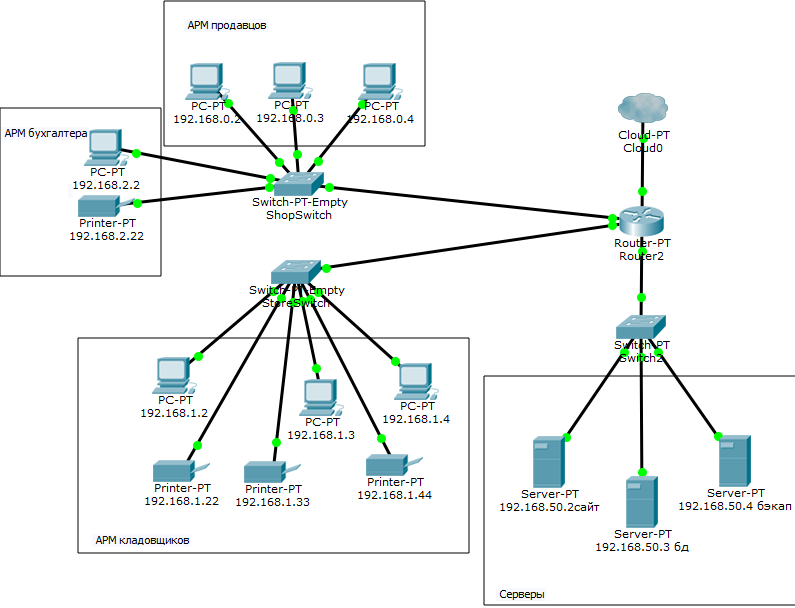
\includegraphics[width=\linewidth]{sec2/img/struct.png}
  \caption{Структурная схема телекоммуникационной системы торгового склада}
  \label{fig:struct}
\end{figure}
